\section{Implementation}
The source for this project (as well as the source code for this report) is available at the git repository hosted publicly at \href{https://github.com/tmplt/ed7039e}{github.com/tmplt/ed7039e}.
If not otherwise specified, any references to a repository shall mean this repository.
Any and all references to files/directories will be to paths relative the repository root.
For example, \texttt{report/} and \texttt{src/lcm-source-dwm.c} refer to \href{https://github.com/tmplt/ed7039e/tree/master/report}{github.com/tmplt/ed7039e/tree/master/report} and \href{https://github.com/tmplt/ed7039e/tree/master/src/lcm-source-dwm.c}{github.com/tmplt/ed7039e/tree/master/src/lcm-source-dwm.c}, respectively.

% We chose to implement our System on a Raspberry Pi.
% This means our system is not in real-time (Linux too complex, other reasons)
% Allows people not versed in embedded systems to write implementations
% A proper implementation would be on a micro-controller that allows code to be run bare-metal, without having to fight with the Linux kernel.

\subsection{Milestones}
The project is divided into four milestones:
\begin{enumerate}
\item \textbf{Two-dimensional navigation:}
  the system should be able to determine its coordinates in a ad-hoc, local grid.
  From its initial position, it should then be able to respond to movement commands on the form ``move to position $(x, y)$''.

\item \textbf{Navigation-line detection:}
  using the subsystem for two-dimensional navigation, the system is to cross a line on the floor,
  thus detecting it and follow it towards the station.

\item \textbf{Station proximity detection, object pickup:}
  once the navigation-line is being followed, the system is to sense when it is sufficiently close to the station to readily use its arm to pick the object up.

\item \textbf{Object displacement, drop-off:}
  after the object has been picked up, the system is to move to another station, find its navigation-line, follow it, and drop the object.
  Note that this milestone is a permutation of the combination of the previous milestones: the same phases should be done in the same order,
  but the system is to move to the second station instead and execute the pickup-process in reverse.
\end{enumerate}

% TODO: write here when each milestone was reached and why it took the time it did

\subsection{Prototyping}
% Here we describe the prototyping stages of the system's components if anything
% out of the ordinary pops up.

\subsubsection{NixOS}
% Introduce NixOS and what is gives us
In this project we have chosen to use NixOS as the operating system on which to run our software.
NixOS is a Linux distibutiton (henceforth referred to as a ``distro'') based upon the Nix package manager (and the terms will be used interchangibly henceforth) that aims to be
\begin{inline-enum}
\item reproducible:
  ``packages [are built] in isolation from each other. [\ldots] they are reproducible and don't have any undeclared dependencies.''\footnote{A positive side-effect of this feature is the complete mitigation of ``dependency hell'': a term relating to a set of problems that commonly arise if multiple versions of a dependency are installed on a system.};
  so if a package works on one machine, it will work on any machine.
  Also, when building a package on multiple machine, all machines will yield the exact same output file tree.
\item Declarative:
  packages are described in expressions that are trivially shared and combined with other package declarations; and
\item reliable:
  ``installing or upgrading one package cannot break other packages''.
\end{inline-enum}~\parencite{nixos.org}

Effectively, NixOS allows us to functionally declare our system in a single (or multiple) expressions ---
that is: Nix enables us to describe the software components of our system in a common manner and how they relate to eachother.
The realization of these expressions can be seen in the repository's \texttt{*.nix} files.
Of particular interest is \texttt{mmc-image.nix}: evaluating this expression generates a bootable image readily flashed onto a MultiMediaCard (MMC)\footnote{Commonly referred to as: SD card, memory card.} that contains the full softare stack and operation instuctions of our robot system.
With the combination of git we can thus version control not only our custom software, but all its dependencies and the complete system behavior.

% How does it differ from a conventional disto?
NixOS is a contrast to the conventional Linux distribution where changes are made to the system via iterative global changes to the system state:
the installation and configuration of software piece-by-piece, for example.
In this mode, it is common to apply ``small changes'' that eventually coalesce into a significant diversion from the originally intended system behavior ---
changes made are not always documented which create a dependency on the ever-changing global state of the system (that is, the file system in which the system is prototyped/implemented).
Of note within this mode is that if the file sysetm is lost, many hours of work may have been wasted if necessary precautions weren't adhered to (by all project members) from the start of the project (such as writing a script that apply all global state changes from a fresh install, for example).
Our usage of NixOS \textit{forces} us to adhere to such precautions.

% What are the negatives of NixOS?
NixOS is no silver bullet, however.
Because of its design, whenever something is to be implemented on NixOS it must be done properly the first time.
Its non-adherence to the Filesystem Hierarchy Standard (FHS)\footnote{the existance and FHS-defined usage of \texttt{/usr}, \texttt{/lib}, \texttt{/var}, and other system directories.} breaks both the build and execution process of many programs.
Unless a program is portably written, it must be patched before it can be used on NixOS where all system files exist under \texttt{/nix/store} which is required to enable the features enumerated in the previous paragraphs.

% Hardware issues
Another problem is the distro's relative infancy to other distros, particularly when it comes to hardware support.
NixOS builds with a generic Linux kernel by default.
A generic kernel is expected to run on a generic system.
Because of the availability of hardware peripherals such as general-purpose input/output pins, GPIO;
universal asynchronous receiver-transmitter, UART;
serial peripheral interface, SPI; and other on the Raspberry Pi we use in this project, our system is not generic.
The result of this is that these peripherals, which we all need, simply do not work.
Fortunately, some work has already been done (and is still being done) by the NixOS community to remedy this.
By applying a so called device-tree overlay on the Linux kernel (and thus describing how an otherwise unknown peripheral may be utilized) SPI was successfully enabled,
which was required to actuate our robot's motors.
Other components we required could be utilized by help of the Raspberry Pi's USB port (fortunately a generic peripheral).
Had we instead opted to use a distro officially supposted by the Raspberry Pi, all of these peripherals would simply work out of the box, but we would then loose the featuses enumerated above.

Some non-generic kernels are offered by NixOS that imply support for Raspberry Pis, but offer none in practise.
The reason for these kernels' availability is presently unknown.

While its certainly possible to enable proper hardware support for all peripherals in the kernel we use, we are on a tight deadline.
As such, we are satisfied even though only SPI is properly supported.

% TODO: what problems does NixOS cause?
% * We cannot use vscode-remote
% * We cannot nix-shell into a shell with ALL appropriate python libs (whatever + brickpi3) because the new env prepends the build one in PATH.
% ...

\subsubsection{Decawave}
This project uses Decawave (or more specifically: a DWM1001 development board) for two-dimensional positioning.
The development board constitutes of the ultra wide-band module itself, the DWM1001C, an accelerometer,
and a Raspberry Pi-compatible GPIO-header.
Via communication over UART, we are able to query its measured position as reported by help of the Decawave anchor nodes\footnote{An anchor is another development board configured for static installation at a known coordinate, used for position calculation. A non-static device with unknown coordinates (as is used in our system) is known as a tag.},
and use this data to figure out where our system is located in the mimicked factory.

% Describe the TLV API we wanted to use.
The device (henceforth referred to as a/the ``DWM'') exposes two modes over UART which we can use to extract data of interest.
One of the modes is a type-length-value (TLV) API which is very suitable for automated interaction:
to extract data using this mode, we need only write three bytes on the form \texttt{\textbf{MSB}}, \texttt{\textbf{MSB-1}}, \texttt{\textbf{MSB-2}}, \texttt{\textbf{...}} where:
\begin{description}
\item[\texttt{MSB}] is the \textit{type} of data we want to send. We specify \texttt{0x40} to call a function via the API.
\item[\texttt{MSB-1}] is the value \textit{value} we want to sent. We specify (for example) \texttt{0x02} to call a function asking for the DWM position.
\item[\texttt{MSB-2}] is the length of the data we want to send. Function \texttt{0x02} takes no payload, so we specifify \texttt{0x00} here.
\item[\texttt{...}] would be a payload of length \texttt{\textbf{MSB-2}} had the function type taken a payload of non-zero size.
\end{description}
One sequece of these bytes constitute a TLV ``frame''.

% Explain the TLV frames, and how nice they are to work with.
After this frame has been written over the serial connection we receive two TLV frames in response:
the first will denote whether the function call was successful (three bytes) and the second the function return data (at least three bytes).
If the first frame says success, we read the next two bytes from which we will know what kind of data the remaining incoming bytes should be interpreted as,
and how much more we should read.
Implementation-wise, always knowing how much data to read allows for performant I/O\footnote{input/output operations: many of which require calling system functions; this is a relatively costly operation.} and easier error handling.
It also allows easy construction of the LCM messages, because they are just a single \texttt{memcpy(3)}\footnote{\texttt{memcpy} - copy memory area: a common operation where a given amount of bytes are copied from a source adress to a destination adress.} away as the byte stream can be trivially represented as a \texttt{struct} following the API documentation.

% No access to acceleration data using the TLV API; generic shell required.
Unfortunately, the TLV API does not expose a function for reading the accelerometer data which we require do estimate the direction of our robot.
A command is, however, readibly available via the interactive shell mode.
This mode instead replies in a human-readable format, but without telling us how many bytes are to be read, and in what way to interpret the data we read.
Fortunately, when the shell is ready to process new input, it writes a ``\texttt{dwm>}'' shell prompt;
we simply read the response until this string is encountered.
This ultimately require us to perform more I/O operations and parse the data upon reception, an operation that is slower than a mere \texttt{memcpy},
but is nevertheless readibly available via a proper call to the \texttt{scanf(3)} family of functions.

An alternative approach where both the TLV API and the shell mode was used was tested but ultimately scrapped:
the time to transition from the TLV API to the shell mode took approximately $1$~s, which broke our $10$~Hz requirement.

\textit{Why} accelerometer data can be queried in one mode but not the other is presently unknown.
We surmise that the existance of the shell mode is for debugging purposes only (because of its human readable format --- and its insistance of using different methods of formatting for similar data types) and that accelerometer data is omitted from the TLV API because it is used by the internal localization functions to detect when the hardware is stationary, or because the developers simply did not foresee this kind of utilization, or both.

Nevertheless, the data we receive when asking for the position is a tuple of
$(x, y, z, q)$, where
\begin{description}
\item[$(x, y, z)$] is the reported coordinate in millimeters in three-dimensional space, and
\item[$q$] is the quality factor: a measure of how sure the device is of the coordinates.
\end{description}

Of note is that the decive cannot approximate its position unless it can connect to at least three anchors.
Additionally, the quality factor, $q$, is higher when connected to four anchors.
During measurements, and if there are more than four anchors available, it will chose the best four anchors to calculate its position. % What does "best" mean here? Refer to documentation.
Because of this, we will then have to consider that our system may suddenly no longer be able fo find its position,
and decide what should be done in order to establish a connection with the disconnected anchors.

Additionally, the data we receive when asking for the acceleration is a tuple of $(x, y, z)$, where
\begin{description}
\item[$(x, y, z)$] is the reported acceleration in three-dimensional space described as raw registers.
\end{description}
% TODO: explain how the register values are calculated to m/s^2

% The data can be considered a random process.

% (X, Y, Z, Q); how is Q calculated?
% What should we do if we cannot connect to 4 anchors at once, a wait?
% Mention that:
% - we have to account for the fact when we tag cannot connect to at least 3 anchors.
% - Qualitative data depends a lot on the positioning of the anchors
% - Built-in 3-axis accelerometer
% - Raspberry Pi compatible GPIO header. Communication via UART.
% - How should we interpset data? It is random proccess? Can we consider noise gaussian?

% TODO:
% RPi UART problems

\subsubsection{BrickPi3}
The BrickPi3 is a peripheral that allows a Raspberry Pi to work with LEGO Mindstorms hardware.
It works by communicating via the SPI function pins of the Raspberry Pi.
The recommended way to install all necessary components is via a \texttt{curl -k | bash}.
There are a few issues with this approach:
\begin{inline-enum}
\item \texttt{-k} is an alias for \texttt{--insecure};
  the recommended approach is thus to not verify the server certificate ---
  this allows a bad actor to feed you malicious code if they have access to your DNS or the target domain.
\item A \texttt{curl | bash} is bad practise for installation purposes as it commonly installs files that are disconnected from the system's package manager.
\item A \texttt{curl | bash} can be detected server-side and thus can conditionally feed a user malicious code.
  A dowload of the code first may thus pass a manual inspection before execution. \parencite{curl-bash}
\end{inline-enum}

Because we use NixOS, the content of the script had to be inspected so that an equivalent Nix expression could be written ---
see \texttt{nix/brickpi3.nix} for the final result.
Upon inspection, a few oddities stood out. The script:
\begin{enumerate}
\item expects and requires the script to be run by the user \texttt{pi}\footnote{Not all users of the peripheral is \texttt{pi}. For example, we use it as \texttt{root} while prototyping.};
\item changes the ownership of a directory with \texttt{sudo(8)} on files under \texttt{/home/pi}, to \texttt{pi}\footnote{In this context, the operations could all have been done as \texttt{pi}.};
\item insecurely downloads multiple scripts and executes them silently --- the downloaded scrips do the same;
\item configures an \texttt{apt(8)} repository (and thus requires to be run on a Debian derivative) for \texttt{npm(1)},
  the Node JavaScript package manager, but never installs or executes any JavaScript packages;
\item installs a C++ source file under \texttt{/usr/local/include}\footnote{A proper installation would be to build a shared library which can then be dynamically linked to when using the C++ drivers.};
\item downloads a precompiled version of \texttt{openocd(1)}, a on-chip debugger and programmer,
  and copies the files into system directories\footnote{No changes are made to the software, according to the mirror's documentation. An installation should instead then be made with the package manager, which is otherwise used in the scripts to install other components}, and then never uses it;
\item runs \texttt{git(1)} as a privileged user, sometimes.
\end{enumerate}
The above list is truncated for sake of brevity.

After a thorough manual inspection of all scripts it was found that only a single Python library (with a single dependency) had to be installed.
The final Nix expression is thus a combination of two \texttt{python3Packages.buildPythonPackage} where both sources are securely downloaded from official mirrors and verified with a known checksum.
We conclude that the usage of this Nix expression leaves the system in a proper state (which the official installation script does not, by oddity 5 and 6\footnote{we consider a proper state of system one in which all installed software components are tracked by the package manager(s).}) and greatly decreases the number of attack vectors with which to run malicious code on our system.

% What need to be done to be able to stack BrickPi3s?

\subsubsection{RobotOS}
% We wanted to use ROS as it was very common to the problem space, and had a lot of readily available solutions for common robot problems.
It was initially decided that the robot system would be implemented with RobotOS (ROS), ``a set of software libraries and tools that help you build robot applications.''\footnote{See \href{https://www.ros.org/}{https://www.ros.org/}.}
The chief reason was its common application in the problem space, its API for communicating different types of messages between different programs\footnote{Known as inter-process communication (IPC).} (in this context known as ``nodes''), and the many readily available solutions to problems we were likely to stumble upon.
% Only officially supports very specific Ubuntu versions, and while probably very applicable to use Nix in this case, it was deemed
% composing ROS on Nix would take too long. (the dependency tree is HUGE)
However, ROS is only officially supported on very specific versions of Ubuntu (at this time of writing), a disto we were not using and a disto that had a very different design philosophies from NixOS;
using ROS on NixOS would thus require a Nix expression to be written that correctly packages the software.
At this point, it was surmised that ROS made several assumption about the global system state that had to be adressed during packaging.
This reason alone would likely require a lot of prototyping time for a simple proof-of-concept execution.
A consultation from another effort to port ROS to an unofficial repository showed that a full desktop installation is constituted of up to 460 packages.\footnote{See \href{https://github.com/ros-noetic-arch}{https://github.com/ros-noetic-arch}, which packages RobotOS to Arch Linux, a distro that is not officially supported by the RobotOS project. Each repository corresponds to a ROS package.}
It was thus decided to find an alternative to RobotOS due to time constrains.

\subsubsection{LCM}
% Trivial to package: just a simple mkDerivation. Nodes are similarly easily packaged. See `nix/software-nodes.nix`.
Lightweight Communications and Marshalling (LCM) ``is a set of libraries and tools for message passing and data marshalling [\ldots] It provides a publish/subscribe message passing model and automatic marshalling/unmarshalling code generation with bindings for applications''.
LCM effectively provides a set of simple functions that enable IPC with the benefit of not requiring a special-purpose daemon (as is required when running ROS).
In difference to ROS, LCM supports any GNU/Linux system (and thus NixOS) and relies on UDP multicasting for broadcasting purposes.
Its short list of dependencies made LCM trivial to package to NixOS: the final expression in \texttt{nix/software-nodes.nix} can be summarized as a \texttt{stdenv.mkDerivation} and the whitelisting of an UDP port in the system firewall.

% Support for C and Python which we have decided to use thus far.
% The core component of ROS we wanted was the message-passing (IPC) component, which this library provides for ANY POSIX-compliant system.
Thus, as LCM:
\begin{inline-enum}
\item enables us to trivially utilize IPC with different message types;
\item has bindings for C and Python; and
\item is trivially packaged,
\end{inline-enum}
it was decided that our robot system would be implemented with help of it in place of ROS.

\subsection{Robot Hardware}
The robot designated the task of moving the object on the industry platform is built from the Lego Mindstorms EV3 core set package. The design of the robot is based from the \cite{Robot arm} model from Legos EV3 core set instructions, but is modified with continuous tracks on the base of the robot, longer arm and some reinforcement to make the robot oscillate less when moving. Instead of using the included \cite{EV3 Intelligent Brick}, a Raspberry Pi 3 together with two BrickPi3 motor shields, see section \ref{brickpi 3}, was used to control the robot. The motors for moving the arm was the EV3 large servomotors \ref{large_servo} and a EV3 servo motor medium \ref{servo_medium} was used for the gripping mechanism.

\subsection{Line Follower}
% GPIO pins does not work. Talk about the dedicated hardware instead.
The docking sequence of the robots movement was implemented using a line follower. A QTRX reflectance sensor from Pololu was used together with a black line to guide the robot close to the factory and to stop it with a perpendicular angle ton the factory(pic). During the project, there occured a connection issue between the Raspberry Pi 4?? and the sensor array due to the fact that no libraries that could transmit data between NixOS and the GPIO pins were found. This issue was resolved by buying an additional breakout board which, in turn, had its own GPIO pins and at the same time could be connected with the Raspberry Pi 3 thru another medium, in this case via a usb-cable. The breakout board used in this project was the Adafruit FT232H Breakout.

\subsubsection{Adafruit FT232H Breakout}
Adafruit FT232H Breakout is a breakout board from Adafruit which contains the F232H chip from FTDI and has has one port each for a usb c and stemma qt male connectors. The board is also equipped with 16 GPIO pins and also has the ability to speak with many protocols including SPI, ITC, serial UART, JTAg and others. In the project, this board was used to transfer GPIO singals from individual sensor on a sensor array to the Raspberry Pi computer. The 
\subsubsection{Sensor Array}
The Sensor array used in this project was a QTRX-MD-16A Reflectance array from Pololu. Each sensor on the sensor array is made from a photo transistor and paired with an IR-led which powers on and keeps emitting light while the sensor array module is powered on. The signal from the photo transistor is transmitted as an analog voltage from the sensor array. 

\newpage
\subsection {Mobile Platform and Trailer}
\subsubsection{Mobile Platform}
A simplified model of the mobile platform can be seen in figure \ref{Mobile_platform_paint}. The power from each motor is transmitted by a beam to three interconnected gears which in turn are inscircled by a rubber band. This configuration  creates two continues tracks powered by one motor each. Due to the fact that each continues track is built in parallel to the platform, the robot is limited to a movement defined by differential drive. As a consequence, the torque in each motor needs to be changed from its initial value in order for the robot to make a turn and change direction from its initial path. 



\begin{figure}[H]
    \centering
    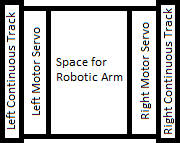
\includegraphics[width = 5 cm]{Mobile_platform_paint.PNG}
    \caption{The Mobile Platform seen from above}
    \label{Mobile_platform_paint}
\end{figure}


\begin{figure}[H]
    \centering
    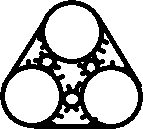
\includegraphics[width = 5 cm]{Band_platform_spikes.PNG}
    \caption{The Mobile Platform seen from the side of one track}
    \label{Mobile_platform_paint}
\end{figure}

\subsubsection{Trailer}
In order to get power to each motor servo and the Raspberry PI, two battery packs with 8 batteries in each were used. Since these battery packs together with the Raspberry Pi and the two BrickPi motorshields were to large to place on the mobile platform, a trailer was built and mounted behind the platform. 

\subsection{Robot arm}
A simplified model of the robot arm can be seen in figure \ref{Arm_model} where the measured distances from \(d_1\) to \(d_7\) and the vertical angle Theta can be seen. in figure \ref{arm_overview} an overview of the robot model can be seen showing how the angle beta was specified.
\begin{figure}[H]
    \centering
    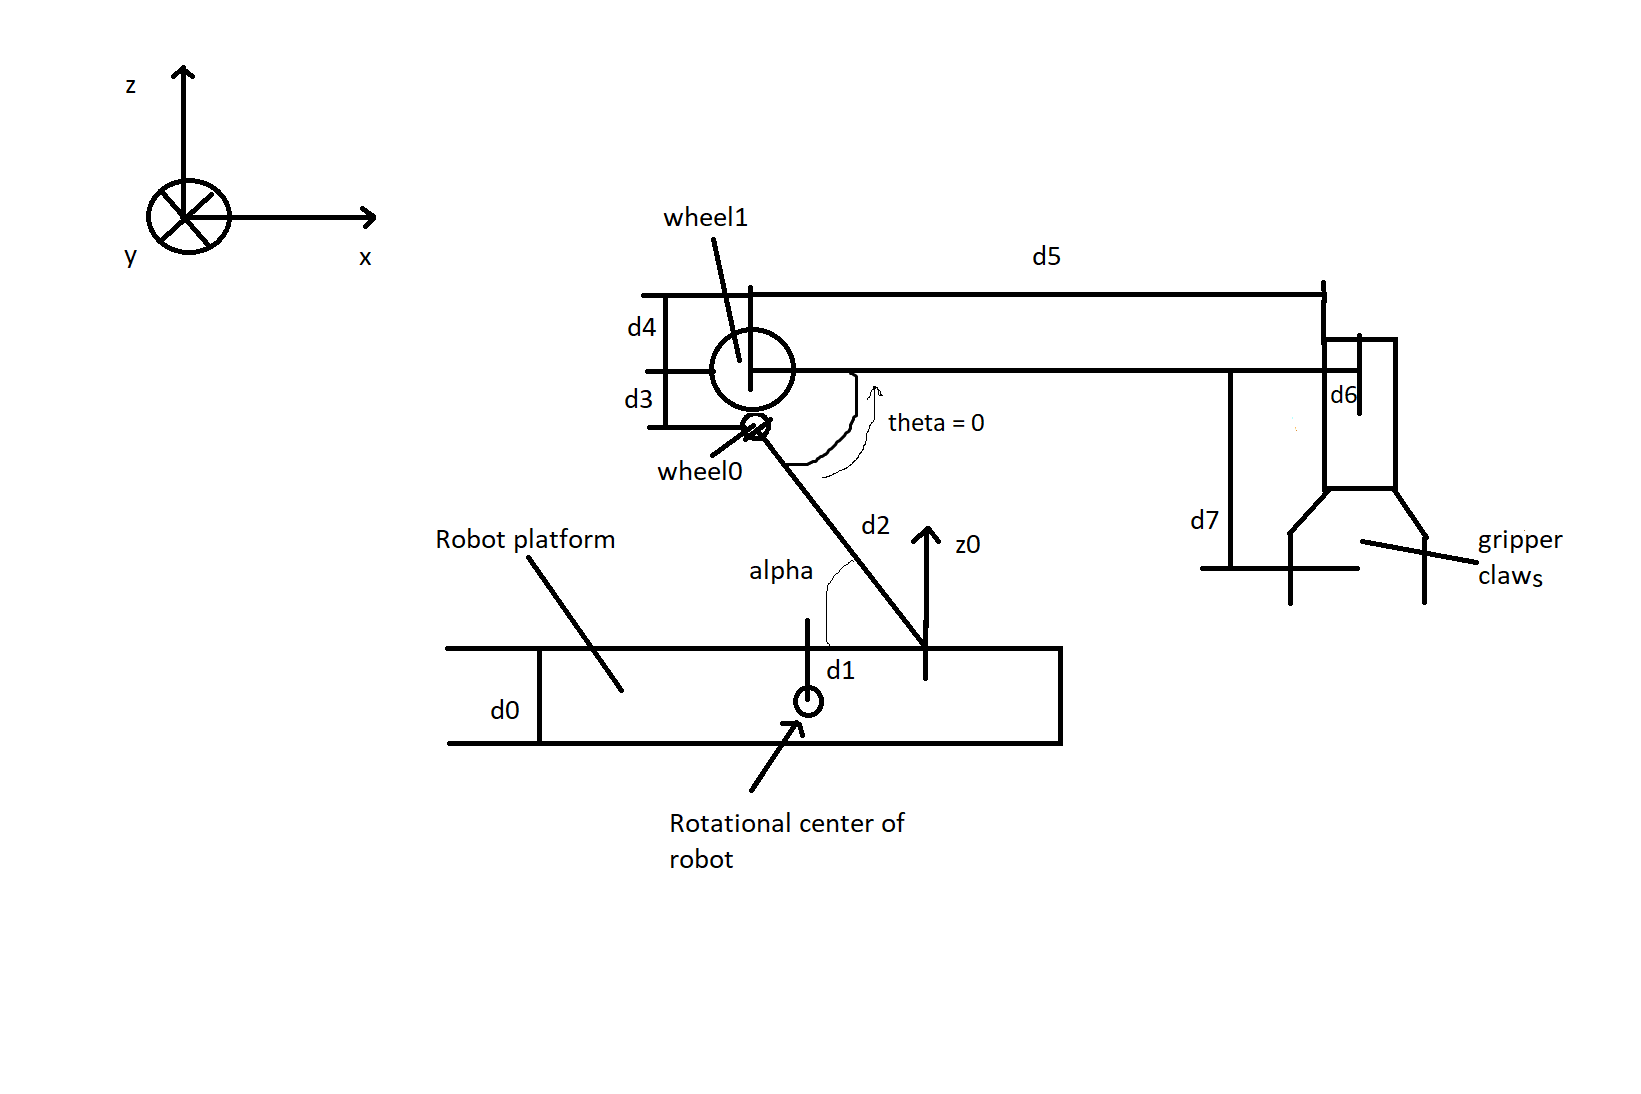
\includegraphics[width = 13 cm]{Arm_model.png}
    \caption{Arm model side view}
    \label{Arm_model}
\end{figure}
\begin{figure}[H]
    \centering
    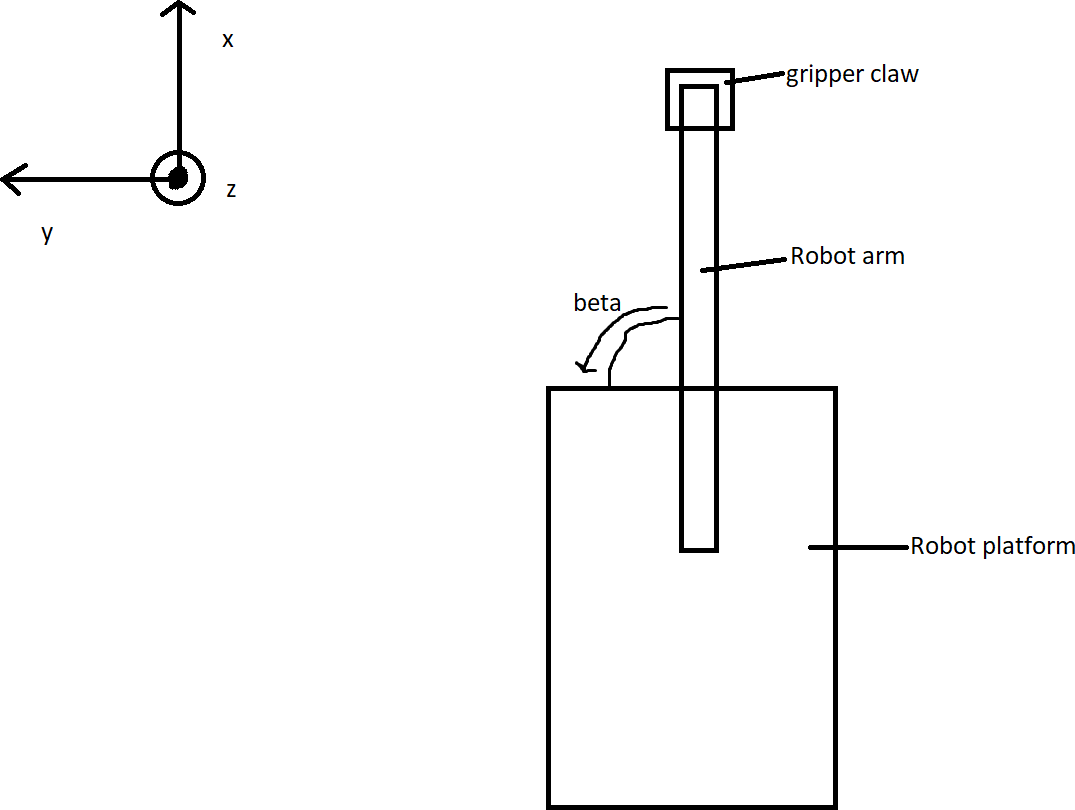
\includegraphics[width = 13 cm]{Arm_overview.png}
    \caption{Arm model overview}
    \label{arm_overview}
\end{figure}
The robot arm can rotate in the xy-plane around the \(z_0\) axis which can be seen in fig. \ref{Arm_model} with a angle Beta using a EV3 large servomotor mounted inside the base of the robot.The upper part of the robot, from wheel1 to the gripper claw can also rotate vertically in the xz-plane using another EV3 large servomotor mounted between wheel0 and the point on the base from where the axis \(z_0\) is originating. The gripper claws  driven with a EV3 servo motor medium since it weighs less. The distances \(d_0\) to \(d_7\) was measured with a ruler and can be seen in table \ref{Tab:distance_table}
\begin{table}[H]
\begin{center}
\begin{tabular}{ |c|c| } 
 \hline
 \(d_0\) & 8 cm  \\ 
 \(d_1\) & 1.5 cm  \\ 
 \(d_2\) & 11.7 cm  \\
 \(d_3\) & 2.2 cm\\
 \(d_4\) & 2.2 cm\\
 \(d_5\) & 23.5 cm\\
 \(d_6\) & 1.5 cm\\
 \(d_7\) & 11 cm \\
 \hline
\end{tabular}
\end{center}
\caption{Table of measured distances \(d_1\) to \(d_7\)}
\label{Tab:distance_table}
\end{table}
\subsubsection{Forward kinematics}
To be able to describe where in the world the gripper claw is, a problem often refereed to as the forward kinematics problem \ref{spong} had to be solved. This was used with a series of homogeneous transformations each representing a change in position and/or orientation relative to what is usually referred to as a frame. The first homogeneous transformation was from the level of the floor to the top of the robot platform, with a distance \(d_0\) which can be seen as a pure translation in the z-direction and can be described as equation \ref{T01} as according to \ref{spong}.
\begin{equation}
    T_{01} = 
    \begin{bmatrix}
    1&0&0&0\\
    0&1&0&0\\
    0&0&1&d_0\\
    0&0&0&1\\
    \end{bmatrix}
    \label{T01}
\end{equation}
then a transformation between the rotational center of the robot to where link \(d_2\) is connected to the base of the robot, which can be expressed as a pure translation in the x-direction. This can be seen in equation \ref{T12}
\begin{equation}
    T_{12} = 
    \begin{bmatrix}
    1&0&0&d_1\\
    0&1&0&0\\
    0&0&1&0\\
    0&0&0&1\\
    \end{bmatrix}
    \label{T12}
\end{equation}
followed by a transformation from the beginning of link \(d_2\) to the center of wheel0. This was done by first making a pure rotation around the z-axis with a angle beta, after which a pure translation in the z-direction with a distance \(d_2\cdot sin(\pi-alpha)\) was made, followed by a translation in the x-direction with a distance \(d_2\cdot cos(\pi - alpha)\) as can be seen in equation \ref{T23}
\begin{equation}
    T_{23} = 
    \begin{bmatrix}
    cos(beta)&-sin(beta)&0&0\\
    sin(beta)&cos(beta)&0&0\\
    0&0&1&0\\
    0&0&0&1\\
    \end{bmatrix}
    \cdot
    \begin{bmatrix}
    1&0&0&0\\
    0&1&0&0\\
    0&0&1&d_2\cdot sin(\pi-alpha)\\
    0&0&0&1\\
    \end{bmatrix}
    \cdot
    \begin{bmatrix}
    1&0&0&d_2\cdot cos(\pi-alpha)\\
    0&1&0&0\\
    0&0&1&0\\
    0&0&0&1\\
    \end{bmatrix}
    \label{T23}
\end{equation}
this was followed by a translation in the z-direction of the distance \(d_3\) between the center of wheel0 to the center of wheel1, see equation \ref{T34}
\begin{equation}
    T_{34} = 
    \begin{bmatrix}
    1&0&0&0\\
    0&1&0&0\\
    0&0&1&d_3\\
    0&0&0&1\\
    \end{bmatrix}
    \label{T34}
\end{equation}
after which a rotation of the coordinate frame in the center of wheel1 was made by an angle -theta around the y-axis and then a translation in the x-direction of the frame in wheel1 by a distance \(d_5 + d6\), see equation \ref{T46}
\begin{equation}
    T_{46} =
    \begin{bmatrix}
    cos(-theta)&0&sin(-theta)&0\\
    0&1&0&0\\
    -sin(-theta)&0&cos(-theta)&0\\
    0&0&0&1\\
    \end{bmatrix}
    \cdot
     \begin{bmatrix}
    1&0&0&d_5 + d_6\\
    0&1&0&0\\
    0&0&1&0\\
    0&0&0&1\\
    \end{bmatrix}
    \label{T46}
\end{equation}
due to the mechanics of the robot model the gripper claw is always pointing straight downwards independent of the angle theta, therefore the coordinate system in the middle if the medium motor connected to link \(d_5\) was rotated back with a positive angle theta before it was translated a distance \(-d_7\) in the z-direction as can be seen in equation \ref{T67}
\begin{equation}
    T_{67} =
    \begin{bmatrix}
    cos(theta)&0&sin(theta)&0\\
    0&1&0&0\\
    -sin(theta)&0&cos(theta)&0\\
    0&0&0&1\\
    \end{bmatrix}
    \cdot
     \begin{bmatrix}
    1&0&0&0\\
    0&1&0&0\\
    0&0&1&-d7\\
    0&0&0&1\\
    \end{bmatrix}
    \label{T46}
\end{equation}
the expression of where the gripper claw can be then expressed as in equation \ref{T_tot} where both it's position and orientation relative to the robot platform is described.
\begin{equation}
    T = T01\cdot T12\cdot T23 \cdot T34 \cdot T46 \cdot T67
    \label{T_tot}
\end{equation}
\subsubsection{Inverse kinematics}
After being able to describe the position and orientation of the gripper it was necessary to have a way of calculating the desired angles theta and beta of the arm to get the gripper claw to a desired position. This problem is often referred to as the inverse kinematics problem. For this robot the angle theta was directly determined by the height of the desired gripper claw position which was calculated according to equation \ref{inv_theta_calc_1} to \ref{inv_theta_calc_5} and the distances \(h_1\) to \(h_3\) can be seen in figure \ref{inv_theta_img}
\begin{figure}[H]
    \centering
    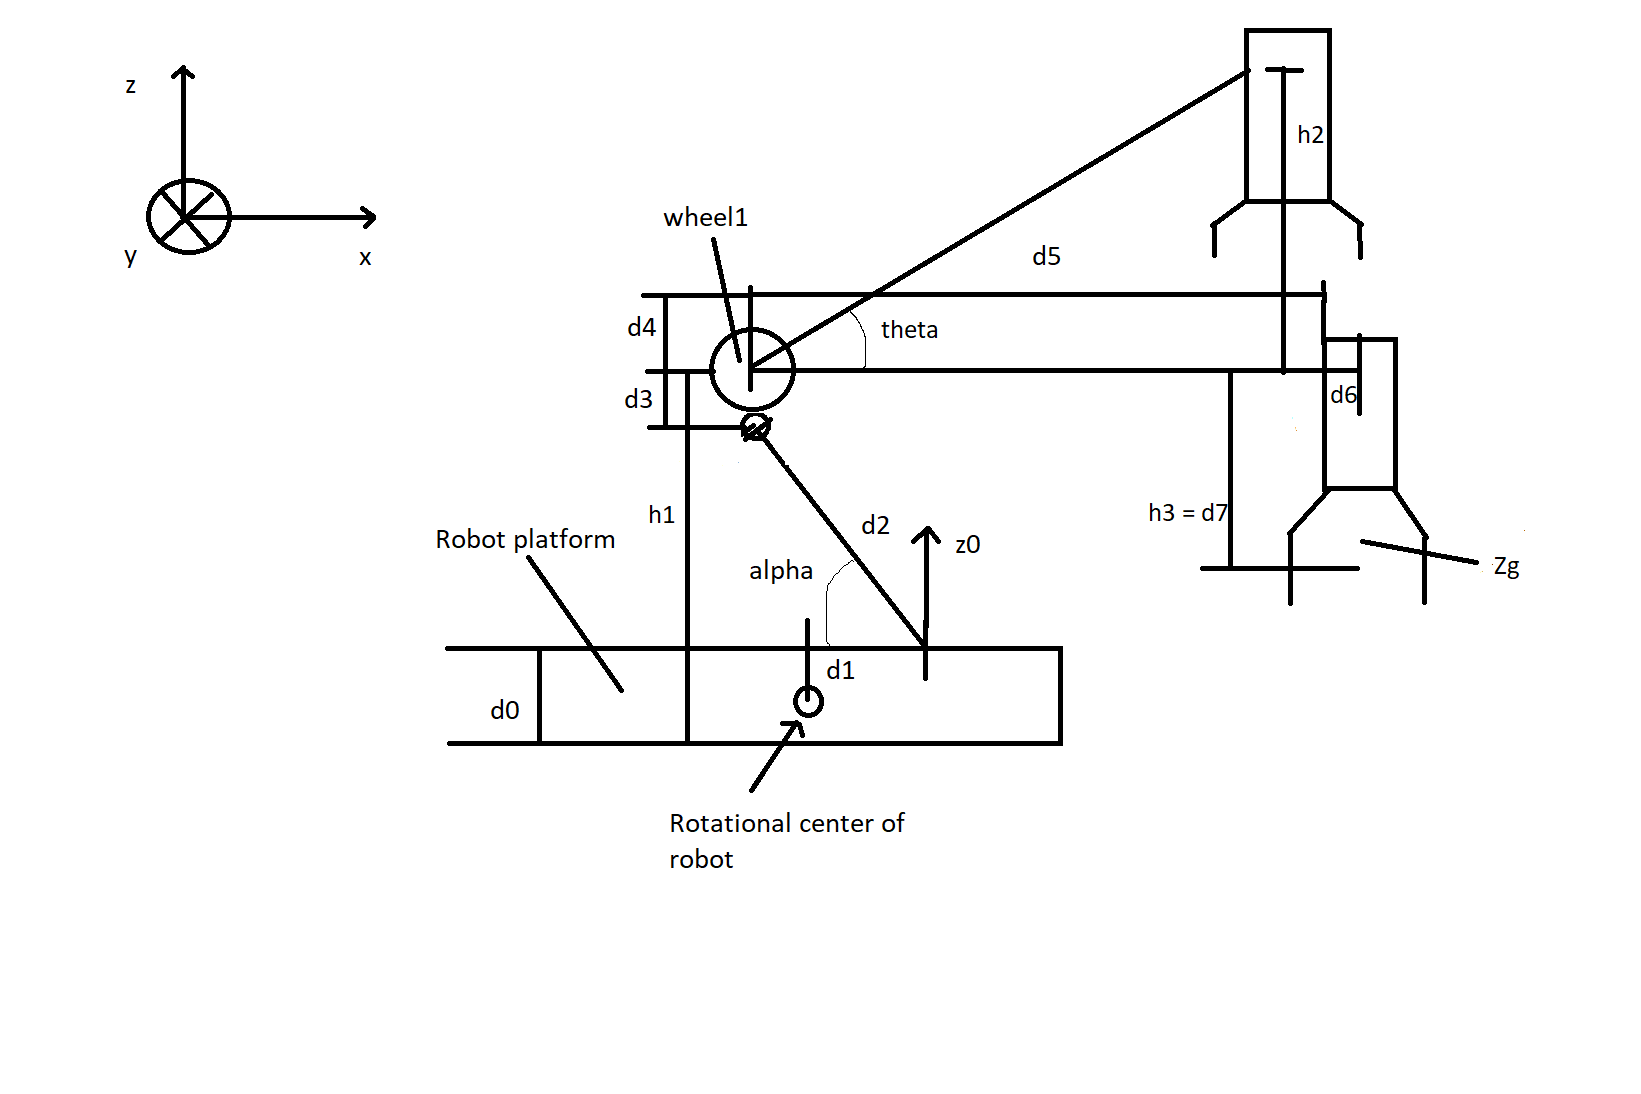
\includegraphics[width = 13 cm]{Arm_model_inv_theta.png}
    \caption{distances \(h_1\) to \(h_3\) on arm model}
    \label{inv_theta_img}
\end{figure}
\begin{equation}
    Z_g = h_1+h_2 - h_3
    \label{inv_theta_calc_1}
\end{equation}
and from figure \ref{inv_theta_img} it can be seen that
\begin{equation}
    h_1 = d_2 \cdot sin(alpha)
    \label{inv_theta_calc_2}
\end{equation}
\begin{equation}
    h_2 = (d_5 + d_6) \cdot sin(theta)
    \label{inv_theta_calc_3}
\end{equation}
\begin{equation}
    h_3 = d_7
    \label{inv_theta_calc_4}
\end{equation}
substituting \(h_1\) to \(h_3\) with expressions from equations  \ref{inv_theta_calc_2} to  \ref{inv_theta_calc_4} the final expression for the angle theta can be solved for in the way that can be seen in equation \ref{inv_theta_calc_5}
\begin{equation}
    theta = sin^{-1}(\frac{Z_g - d_2 \cdot sin(alpha) + d7}{(d_5 + d_6)})
    \label{inv_theta_calc_5}
\end{equation}
Since the arm could rotate horizontally it could reach points on a circle, see figure \ref{inv_beta_radius_img}, around itself where the radius of that circle, with the rotational center of the robot being the center of the circle, depended on the angle theta in a way that is described in equation \ref{beta_radius_eq}.
\begin{figure}[H]
    \centering
    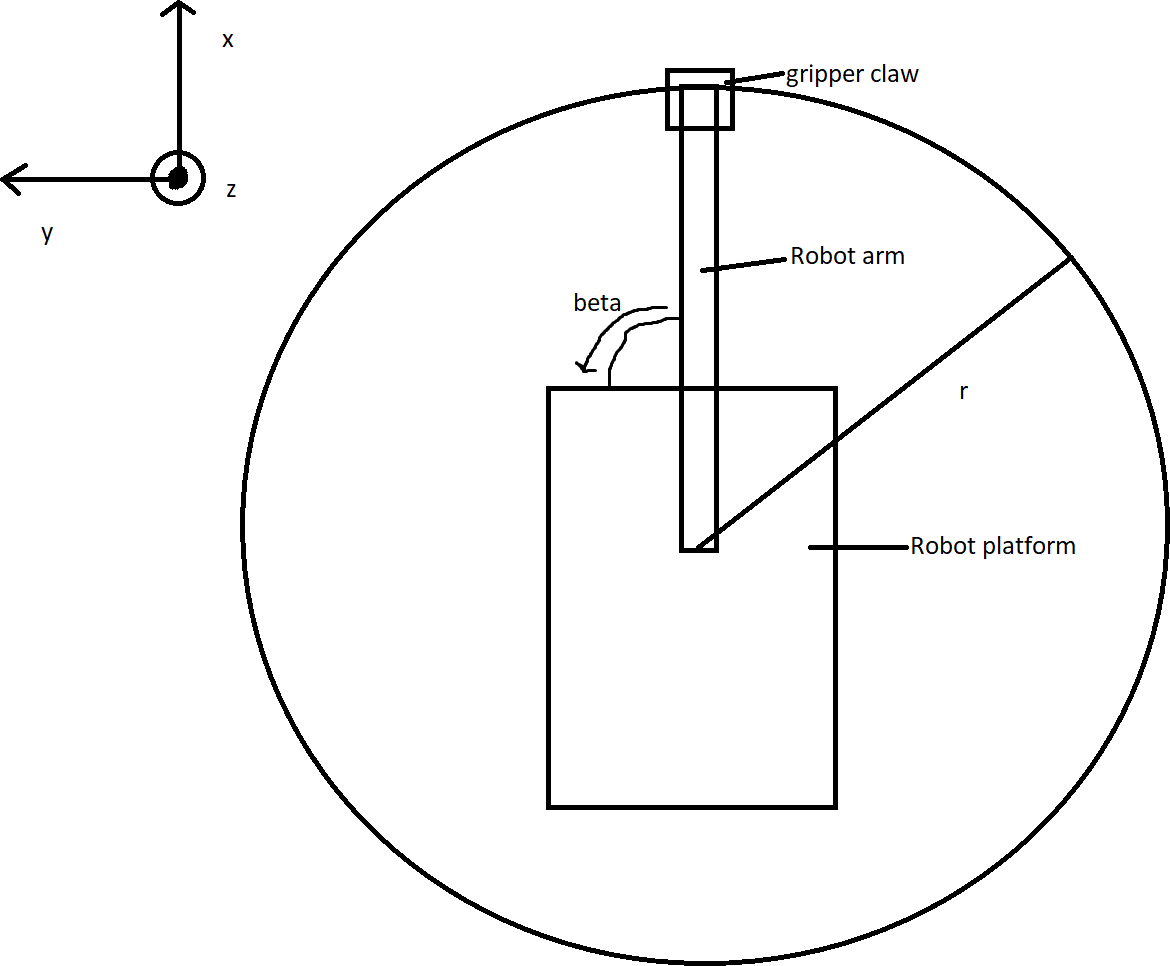
\includegraphics[width = 13 cm]{inv_beta_radius.png}
    \caption{distances \(h_1\) to \(h_3\) on arm model}
    \label{inv_beta_radius_img}
\end{figure}
\begin{equation}
    r = (d_5 + d_6)\cdot cos(theta) - d_2\cdot cos(alpha) + d_1
    \label{beta_radius_eq}
\end{equation}
calculations of x and y positions on a circle can be seen in equations \ref{circle_x} and \ref{circle_y}
\begin{equation}
    x = r\cdot cos(beta)
    \label{circle_x}
\end{equation}
\begin{equation}
    y = r\cdot sin(beta)
    \label{circle_y}
\end{equation}
substituting r to the expression from equation \ref{beta_radius_eq} the calculations of the x and y positions on the circle around the robot can be seen in equations \ref{circle_x_robot} and \ref{circle_y_robot}
\begin{equation}
    x = ((d_5 + d_6)\cdot cos(theta) - d_2\cdot cos(alpha) + d_1)\cdot cos(beta)
    \label{circle_x_robot}
\end{equation}
\begin{equation}
    y = ((d_5 + d_6)\cdot cos(theta) - d_2\cdot cos(alpha) + d_1)\cdot sin(beta)
    \label{circle_y_robot}
\end{equation}
solving for beta in equations \ref{circle_x_robot} and \ref{circle_y_robot} the following expressions was achieved 
\begin{equation}
    beta = cos^{-1}(\frac{x}{(d_5 + d_6)\cdot cos(theta) - d_2\cdot cos(alpha) + d_1})
    \label{Beta_x_robot}
\end{equation}
\begin{equation}
    beta = sin^{-1}(\frac{y}{(d_5 + d_6)\cdot cos(theta) - d_2\cdot cos(alpha) + d_1})
    \label{Beta_y_robot}
\end{equation}
these two expressions both have a denominator which is equal to zero for an angle \(theta = \pm \pi /2\), two angles that the robot can never reach due to the way the Lego hardware is put together.\\
From equations \ref{Beta_x_robot} and \ref{Beta_y_robot} it is clear that only the desired x or the y position was needed to calculate beta, in this project the x positions were used.\newpage
\subsubsection{Resolution}
As mentioned before the motors used in the robot arm was two Lego EV3 servo motor large for making the arm move vertically and horizontally and one Lego EV3 servo motor medium inside the gripper to pick up boxes on the miniature industry platform. Both the Large and the medium motors had a resolution of 1 degree, meaning the motors gives 360 readings on one revolution. Also on the robot the cogwheel attached to the motor controlling vertical movement on the arm, see wheel0 in figure \ref{Arm_model}, was connected to another cogwheel, see wheel1 in figure \ref{Arm_model}, which had 5 times as many teeth giving 5 times higher resolution for the arm itself than the motor in vertical movement. In the same way the cogwheel attached to the motor controlling horizontal movement of the arm was connected to another cogwheel with 3 times as many teeth giving 3 times higher resolution for the arm relative to the motor in horizontal movement.
\subsubsection{Initialization}
There is no memory in the motors which makes the robot "unaware" of the original orientation of the arm on boot. Therefore an initialization process was made for the robot using two Lego EV3 touch sensors \ref{touch_sensor}. On boot the robot moved the arm with constant angular speed, in the beta direction, until a lego piece, moving with the arm, pressed one of the touch sensors at \(beta = -90^{\circ}\) then it stopped moving in that direction. In the same way the robot moved the arm in the positive theta direction until another lego piece getting closer to the other touch sensor with an increasing beta angle, pressed the second touch sensor at \(theta = 36^{\circ}\). then it stopped in that direction. At the point when both touch sensors was pressed and the arm had stopped moving in both directions the position of the arm was known.\newpage
\subsection{Robot software}
Two BrickPi3 motor shields were used to drive the motors and sensors on the robot. A complete library for controlling lego motors and sensors connected to the motor shields were developed by the manufacturers of the BrickPi3 together with the shields and was used to control the motors. Additionally P, PI and PID controllers was developed in this project to compare functions in the BrickPi3 library for controlling the motors and the movement on the arm.
\subsubsection{P controller}
A P controller, or proportional controller, is a feedback control structure where the output error is fed back to the motors to make them act proportional to the error. In the P controller made for controlling the movement on the robot arm an angular error was expressed, see equation \ref{ang_err}
\begin{equation}
    e_{\theta} = \theta_{desired} - \theta
    \label{ang_err}
\end{equation}
where \(\theta\) is the current angular position of the arm and \(\theta_{desired}\) is the goal angle. The angular error was then fed back to the motors to make them act on it is a way that can be seen in equation \ref{P_control}
\begin{equation}
    P = K_p\cdot e_{\theta}
    \label{P_contol}
\end{equation}
where P is motor speed, proportional to the angular error and \(K_p\) is a proportional gain which determines how aggressive the controller should be.\\

\subsubsection{PI controller}
A PI controller or proportional integral controller is a proportional controller to which a term which integrates the error over time is added. The integration was done in a discrete fashion where, in every loop of the robot arm code running, the new calculated error was added to a integral error term, see equation \ref{integral_term}
\begin{equation}
    e_{integral} = e_{integral} + e_{\theta}
    \label{integral_term}
\end{equation}
where \(e_{integral}\) is the discrete approximation of the integrated error, \(e_{\theta}\) is the same as in equation \ref{ang_err}. This error was adding up over time and the feedback to the motors can be seen in equation \ref{PI_control}
\begin{equation}
    P = K_p\cdot e_{\theta} + K_i\cdot T_s\cdot e_{integral}
    \label{PI_control}
\end{equation}
where P is the motor speed, \(T_s\) is the sampling period of the code to make the integral term normalized in a sense, and \(K_i\) is the integral gain which determines how much the motors should act on the integral error.

\subsubsection{PID controller}
A PID or proportional integral derivative controller is a control structure where both a proportional, integral, and a derivative term is added. The differentiation was also done in a discrete fashion and was approximated as in equation \ref{derivative_term}
\begin{equation}
    e_{diff} = e_{old} - e_{\theta}
    \label{derivative_term}
\end{equation}
where \(e_{diff}\) is the discrete approximation of the differentiated error, \(e_{old}\) is the old error from the previous loop of the code and \(e_{\theta}\) is the same as in equation \ref{ang_err}. The feedback to the motors was done according to equation \ref{PID_control}
\begin{equation}
    P = K_p\cdot e_{\theta} + K_i\cdot e_{integral} + K_p\cdot e_{diff}
    \label{PID_control}
\end{equation}
\subsubsection{Tuning of the controllers}
The tuning of the controllers was made with a Ziegler Nichols approach, see \ref{Ziegler}, since a development of a dynamic model of the arm was not completed. The Ziegler Nichols tuning method required two measured parameters to be found. First the Oscillation gain which is the gain of a proportional controller \(K_p\) for which the output of the system acting on a step response is undamped oscillations. This was found by making the robot arm act on a step response several times while changing the value of the proportional gain \(K_p\). The second measured parameter is the oscillation time \(T_{osc}\), e.g the time it takes for the system to make one undamped oscillation period. This was found by looking at a plotted graph of the undamped oscillations and counting the measured values in one period. The calculations of the oscillation time could then be done as shown in equation \ref{osc_time}
\begin{equation}
    T_{osc} = n\cdot T_s
    \label{osc_time}
\end{equation}
where \(T_{osc}\) is the oscillation time, n is the number of measured values in one undamped oscillation period from the output of the step response and \(T_s\) is the sampling period of the robot.
\subsection{Software nodes}
% Here we'll summarize each node
Each node follow the naming scheme of \texttt{lcm-<type>-<desc>.<ext>} where
\begin{description}
\item[\texttt{<type>}] denotes the type of three possible alternatives:
  \texttt{source}, which denotes that the node only provides messages to the system;
  \texttt{sink}, only receives messages from the system; and
  \texttt{int} (for `intermediate'), both receives and generates messages.
\item[\texttt{<desc>}] is a list of words interspaced by a \texttt{-} that provide a short description of the node's purpose.
\item[\texttt{<ext>}] is the source file extension. It describes how the node should be built before it can be executed.
  For example, if the extension is \texttt{c} then the node was written and C and needs to be compiled and linked with a C compiler before the resulting binary can be executed.
  If the extention instead is \texttt{py} then the node was written in Python, and nothing must be done before the script can be executed.
\end{description}

The source files for all nodes can be found in \texttt{src/}.

\subsubsection{\texttt{lcm-source-dwm.c}}
This node is responsible for extracting the position and acceleration data from the DWM.
Upon execution it opens opens a serial communication to the DWM, enters the shell mode and allocates a buffer into which received data is read into.
Afterwards it enters a loop within which the shell commands \texttt{av} is continously called.
While spinning in this loop, the node keeps the time and ensures that the command \texttt{apg} is called with a frequenzy of $10$~Hz.
After the execution of each command:
\begin{enumerate}
  \item the response is read into the buffer;
  \item the buffer is parsed for data of interest;
  \item data is converted to SI units --- m for position coordinates, $\text{ms}^{\text{-2}}$ for acceleration; and
  \item an appropriate message type is constructed and published to all subscribing nodes.
\end{enumerate}

\subsubsection{\texttt{lcm-source-robot-target.py}}
This node simply provides a target coordinate, relative to the grid established by the DWM, that the robot should move to.
